\documentclass[11pt]{jarticle}
% \usepackage[a4paper,hmargin=20mm,vmargin=15pt]{geometry}
% \usepackage{amsmath}
% \usepackage{amsthm}
% \usepackage{amssymb}
\usepackage[dvipdfmx]{graphicx}
\usepackage{tikz}
\pagestyle{plain}
\begin{document}
\title{}
\date{}
\author{}
\maketitle
\paragraph{問題4.}
(1) $(a_1, a_2, a_3)$の組み合わせとして起こりうるものと
それらが持つサイクルは, 
\begin{align*}
  (1, 2, 3) \quad a_1=& 1,\quad a_2= 2,\quad a_3= 3 \\
  (1, 3, 2) \quad a_1=& 1,\quad a_2= 3 \to a_3= 2 \\
  (2, 1, 3) \quad a_1=& 2 \to a_2= 1,\quad a_3= 3 \\
  (2, 3, 1) \quad a_1=& 2 \to a_2= 3 \to a_3= 1 \\
  (3, 1, 2) \quad a_1=& 3 \to a_3= 2 \to a_2= 1 \\
  (3, 2, 1) \quad a_1=& 3 \to a_3= 1,\quad a_2= 2
\end{align*}
である. このうち, $(1,2,3), (1,3,2), (2,1,3), (3,2,1)$が長さ$1$のサイクルを持つ. 
従って求める確率は, 
\begin{equation*}
  \frac{4}{6} = \underline{\frac{2}{3}}
% by 杉原宇宙(061700950) as s-sugihara%
\end{equation*}
(2)$n = 4$のとき長さ$4$のサイクルは相異なる$i, j, k, l \in \{ 1, 2, 3, 4 \}$を用いて以下のように表せる. 
\begin{equation*}
  a_{i} = j \to a_{j} = k \to a_{k} = l \to a_{l} = i
\end{equation*}
ここで$ i, j, k, l $の組み合わせは, 
\begin{equation*}
  (i, j, k, l) = (1, 2, 3, 4), (1, 2, 4, 3), (1, 3, 2, 4), (1, 3, 4, 2), (1, 4, 2, 3), (1, 4, 3, 2)
\end{equation*}
の6通りである. よって長さ$4$のサイクルを含む順列は以下のものである. 
\begin{equation*}
  (2, 3, 4, 1), (2, 4, 1, 3), (3, 4, 2, 1), (3, 1, 4, 2), (4, 3, 1, 2), (4, 1, 2, 3) 
\end{equation*}
% by 高野匠(061701051) as ttt-takano%
(3) \ $x>0$において, $f(x)=\frac{1}{x}$は単調減少. \\
また, $n$以下の正の整数$k$に対して, $k\leqq x\leqq k+1$のとき, $f(x)\leqq f(k)$ \\
以上より, 下図から面積を比較して, \\
\begin{equation*}
  \sum_{j=k}^{n} \frac{1}{j} 
  > \int_{k}^{n+1} \frac{1}{x} \ dx 
  = \left[ \log x \right]_{k}^{n+1}
  = \log (n+1) - \log k
\end{equation*}
よって, 題意は示された. \hfill $\Box$ \\
\begin{center}
  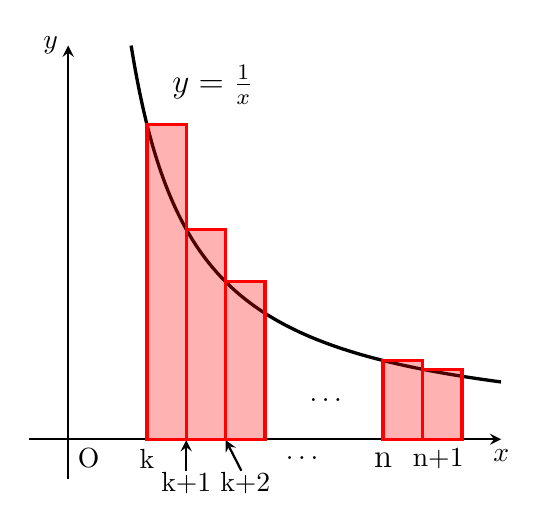
\begin{tikzpicture}
    
    % 座標軸
    \draw [thick, -stealth](-0.5,0)--(5.5,0) node [anchor=north]{$x$};
    \draw [thick, -stealth](0,-0.5)--(0,5) node [anchor=east]{$y$};
    \node [anchor=north west] at (0,0) {O};
  
    % y=1/x
    \draw [very thick, domain=0.8:5.5, samples=200] plot(\x, 4/\x);
    \node [anchor=west] at (1.2,4.5) {\large $y=\frac{1}{x}$};
  
    % 長方形(j=k)
    \draw [very thick, draw=red] (1,0) rectangle (1.5,4);
    \fill [red, opacity=.3] (1,0) rectangle (1.5,4);
    \node [anchor=north] at (1,0) {k};
  
    % 長方形(j=k+1)
    \draw [thick, -stealth](1.5,-0.4)--(1.5,-0.01);
    \draw [very thick, draw=red] (1.5,0) rectangle (2,4/1.5);
    \fill [red, opacity=.3] (1.5,0) rectangle (2,4/1.5);
    \node [anchor=north] at (1.5,-0.3) {k+1};
  
    % 長方形(j=k+2)
    \draw [thick, -stealth](2.2,-0.4)--(2.0,-0.01);
    \draw [very thick, draw=red] (2,0) rectangle (2.5,2);
    \fill [red, opacity=.3] (2,0) rectangle (2.5,2);
    \node [anchor=north] at (2.25,-0.3) {k+2};
  
    % 長方形(k=n)
    \draw [very thick, draw=red] (4,0) rectangle (4.5,1);
    \fill [red, opacity=.3] (4,0) rectangle (4.5,1);
    \node [anchor=north] at (4,-0.05) {\large n};
  
    % 長方形(k=n+1)
    \draw [very thick, draw=red] (4.5,0) rectangle (5,4/4.5);
    \fill [red, opacity=.3] (4.5,0) rectangle (5,4/4.5);
    \node [anchor=north] at (4.7,0) {n+1};
  
    % …の挿入
    \node at (3.3,0.5) {\ldots};
    \node [anchor=north] at (3.0,-0.1) {\ldots};
    
  \end{tikzpicture}
  \\
  \textgt{図}\quad $y=\frac{1}{x}$のグラフと長方形
\end{center}
% by 大橋知生(061700353) as FulminicAcid %
\end{document}